\subsection{Interpretability}

\begin{frame}{What Is the Model Looking At?}
  \scriptsize
  \begin{itemize}
    \item GradCAM applied to \textbf{both} branches (spatial and frequency) for \textbf{both} heads: is a prediction driven by texture cues or by spectral artifacts?
    \item Spatial-branch heatmaps localize tightly on the main subject; frequency-branch heatmaps vary sample to sample rather than firing on a fixed region.
    \item Samples now drawn from a fixed (non-shuffled) validation order, so examples reproduce across runs.
  \end{itemize}

  \vspace{-.2em}
  \centering
  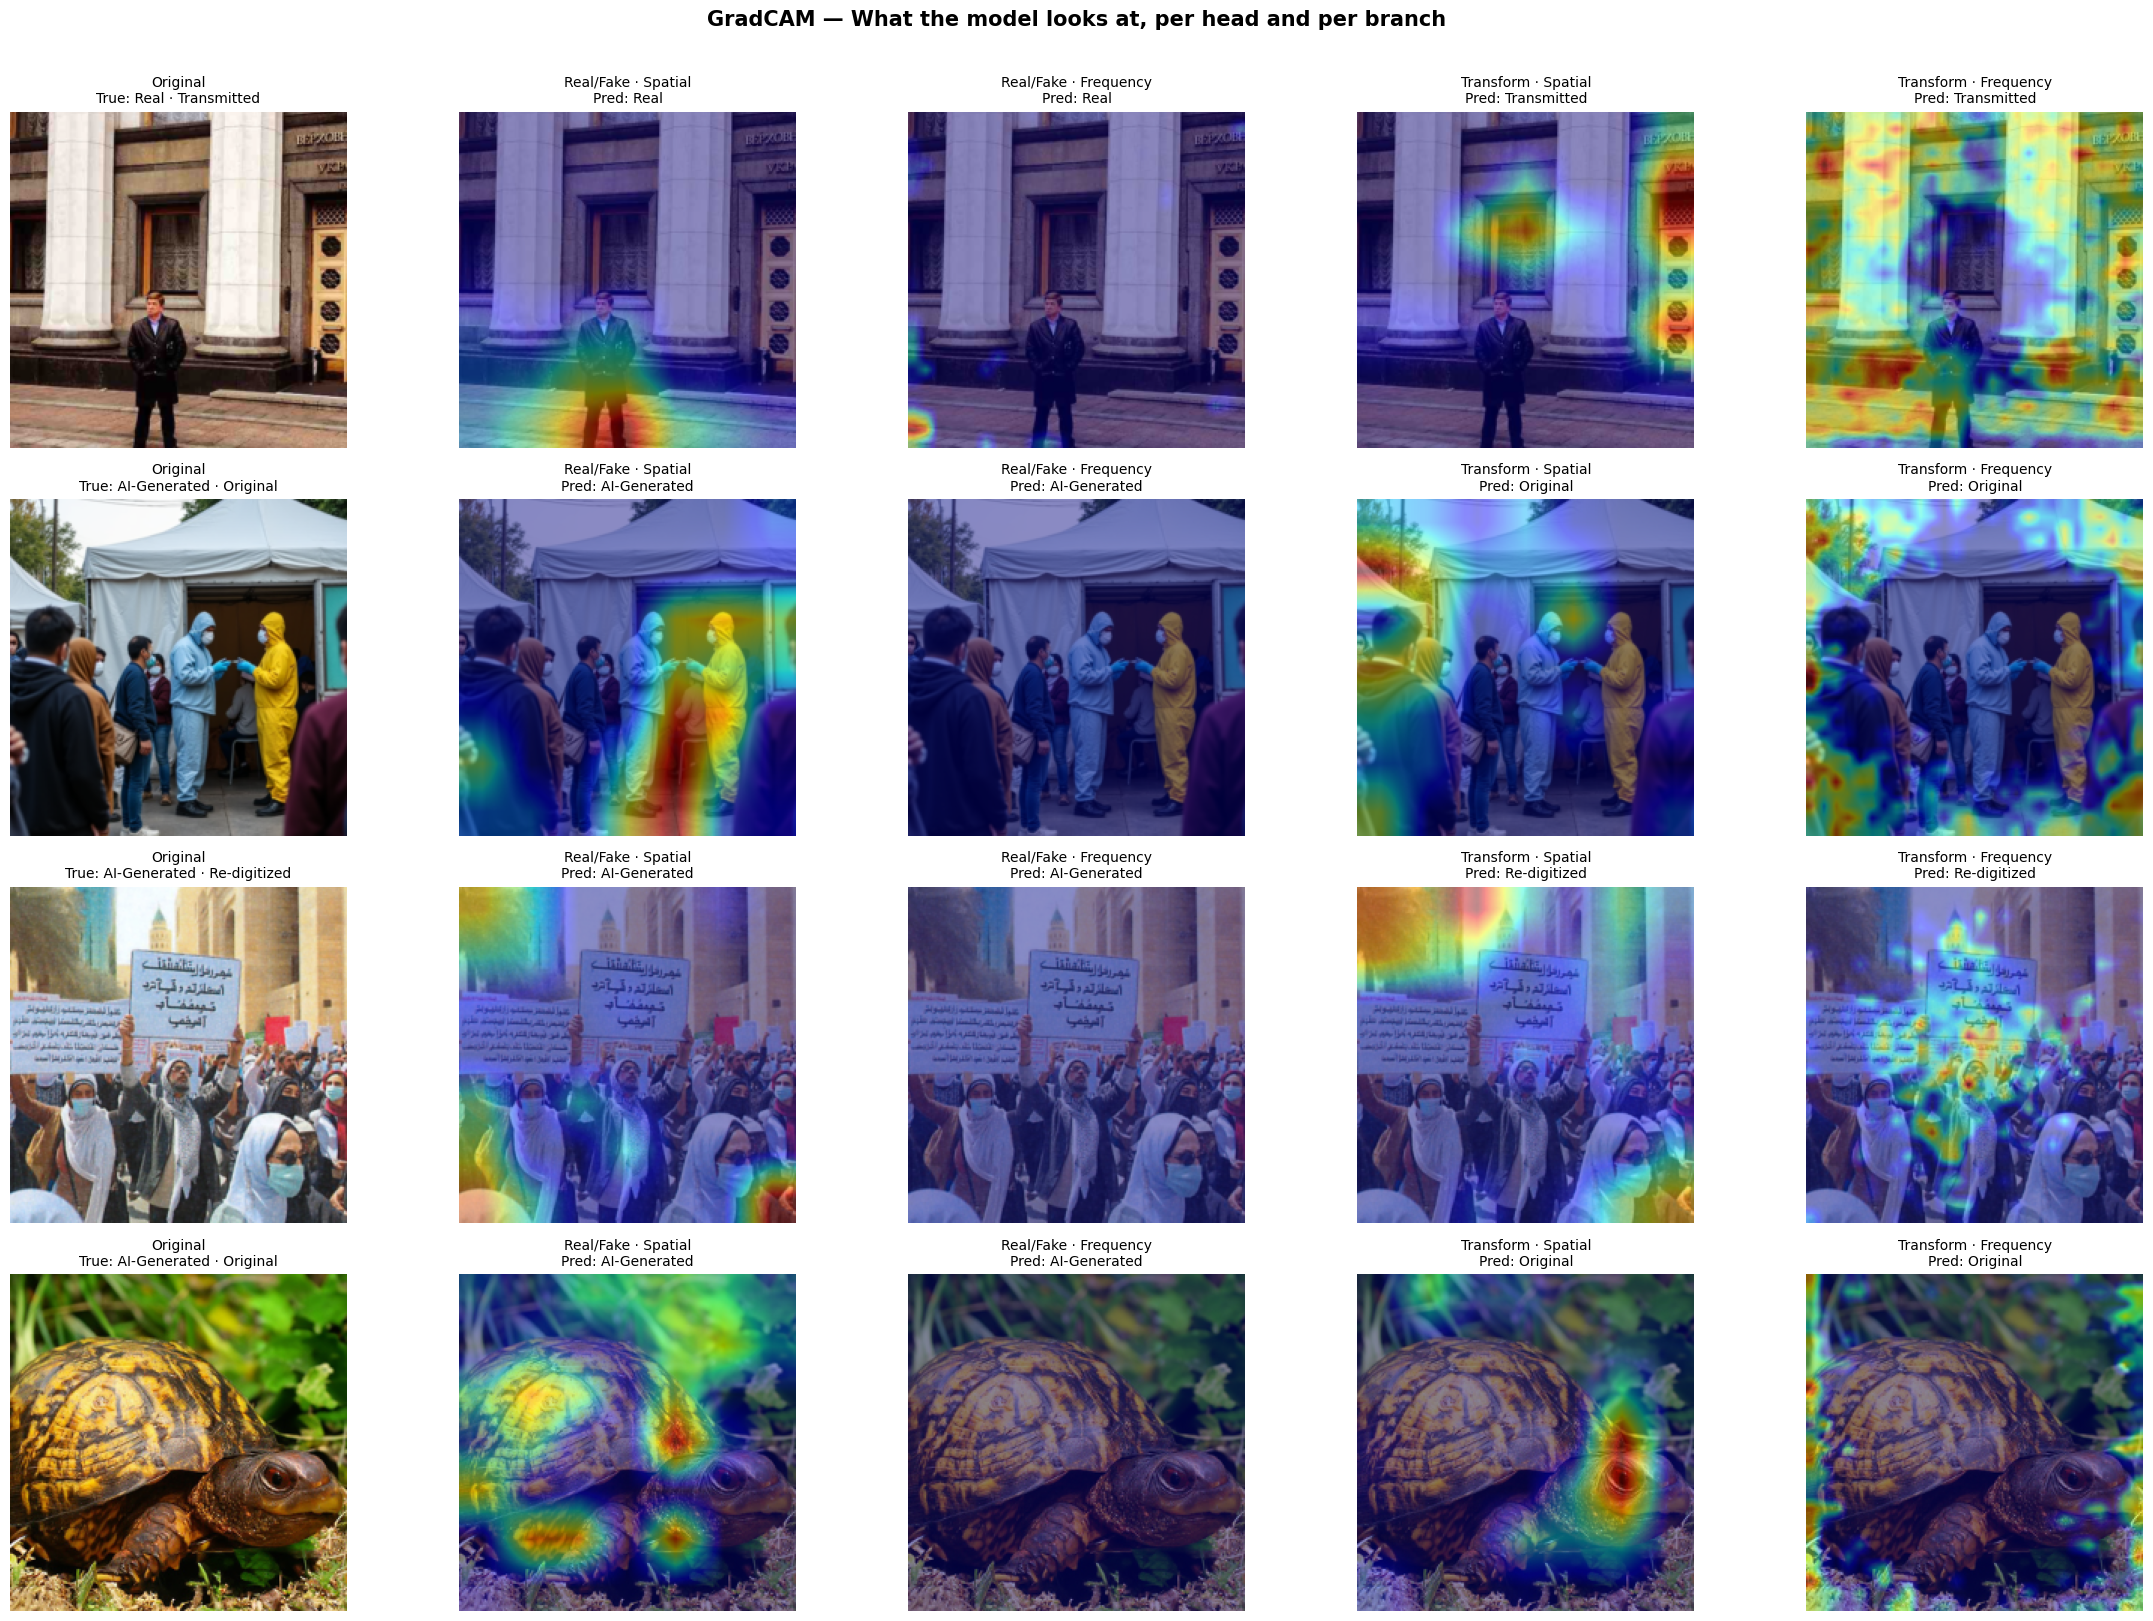
\includegraphics[height=4.6cm]{assets/gradcam.png}
\end{frame}
